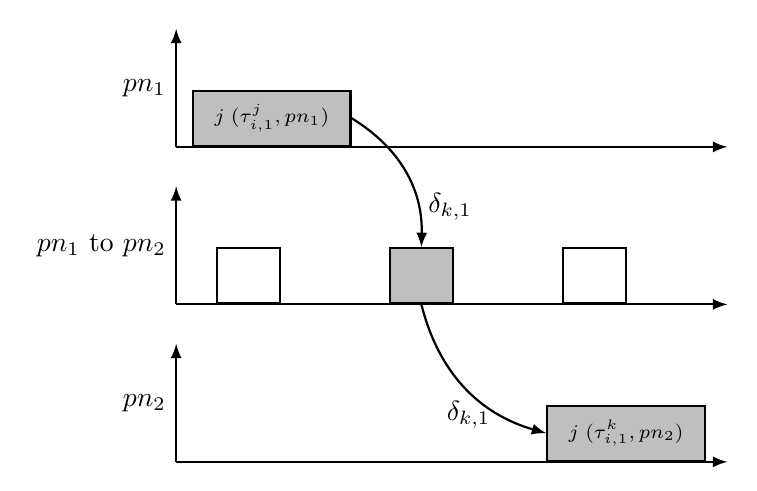
\begin{tikzpicture}
    \draw[thick, -latex] (0,0) -- (7,0); 
    \draw[thick, -latex] (0,2) -- (7,2); 
    \draw[thick, -latex] (0,4) -- (7,4); 
    \draw[thick, -latex] (0,0) -- (0,1.5) node[midway, left] {$pn_2$}; 
    \draw[thick, -latex] (0,2) -- (0,3.5) node[midway, left] {$pn_1$ to $pn_2$}; 
    \draw[thick, -latex] (0,4) -- (0,5.5) node[midway, left] {$pn_1$};

    \draw  (0.2,4) node[draw, thick, fill=lightgray, rectangle, anchor=south west, inner sep=0pt, minimum width=2cm, minimum height=0.7cm] (jpn1) { \scriptsize $ j \; ( \tau_{i,1}^j, pn_1 )$};
    \draw  (4.7,0) node[draw, thick, fill=lightgray, rectangle, anchor=south west, inner sep=0pt, minimum width=2cm, minimum height=0.7cm] (jpn2) { \scriptsize $ j \; ( \tau_{i,1}^k, pn_2 )$};

    \draw  (0.5,2) node[draw, thick, fill=white, rectangle, anchor=south west, inner sep=0pt, minimum width=0.8cm, minimum height=0.7cm] {};
    \draw  (2.7,2) node[draw, thick, fill=lightgray, rectangle, anchor=south west, inner sep=0pt, minimum width=0.8cm, minimum height=0.7cm] (dpc) {};
    \draw  (4.9,2) node[draw, thick, fill=white, rectangle, anchor=south west, inner sep=0pt, minimum width=0.8cm, minimum height=0.7cm] {};
    \draw (jpn1.east) edge[thick, -latex, bend left] node[near end, right] {$\delta_{k,1}$} (dpc.north);
    \draw (dpc.south) edge[thick, -latex, bend right] node[near end, left] {$\delta_{k,1}$} (jpn2.west);
\end{tikzpicture}
